\documentclass[conference]{IEEEtran}  % Usa lo stile IEEE per impaginazione a 2 colonne
\usepackage[utf8]{inputenc}
\usepackage{graphicx}
\usepackage{caption}  
\usepackage{subcaption} 
\graphicspath{{Figures/}} 
\usepackage{amsmath}
\usepackage{cite}
\usepackage{hyperref}
\usepackage{amssymb}


\title{Can We Detect The Fake Music Generator\\ From The Description Of The Music?}
\author{
    \IEEEauthorblockN{Andrea Paglialunga, Alice Portentoso, Bian Lei}
    \IEEEauthorblockA{
        Dipartimento di Elettronica, Informazione e Bioingegneria (DEIB), Politecnico di Milano \\
        Music and Acoustic Engineering (MAE), Politecnico di Milano \\
        }
}

\begin{document}

\maketitle

\begin{abstract}
\textit{Text-To-Music (TTM)}
The advances in AI-driven music generation require robust and reliable methods to attribute generated content to its source. 

The advent of Text-to-Music (TTM) models marks a significant advancement in the field of automatic music generation. These models have achieved unprecedented performance levels.
TTMs are experiencing rapid adoption in commercial applications and contemporary music production workflows. 

However, this pervasive integration introduces pressing concerns related to copyright infringement, intellectual property, and the accurate attribution of generated content. These issues require rigorous investigation by the audio forensic and broader research communities.

The core objective of this research is to develop and evaluate a robust text classification framework capable of distinguishing between the different generators, so identifying the generative model behind a given music caption. This work aims to contribute to the development of methodologies for content provenance and attribution in the evolving landscape of AI-driven creative media.

\end{abstract}


\begin{IEEEkeywords}
Audio Captioning, Text Classification, Audio Forensics, BERT, Fine-tuning, Open-Set Recognition.
\end{IEEEkeywords}

\section{Introduction}
Advancements in text-to-music models, such as Magenta \cite{zhu2023surveyaimusicgeneration}, have made AI-generated music nearly indistinguishable from human compositions. This progress raises important ethical, sociological, and political concerns \cite{afchar2025aigeneratedmusicdetectionchallenges}.

AI technologies often rely on huge datasets that contain already existing work. This raises questions regarding the unauthorized use of original material and the violation of copyright, especially if AI reworks protected content without the authors' consent.
The generation of music through AI tends to rely on predefined patterns and models, risking the creation of a homogeneous musical landscape where the pieces are similar to each other. This limits the innovation and creative diversity that arises from human experience and uniqueness.

So, the fundamental question that arises in this context is:
"If music is generated using models conditioned on text, can we caption the audio and use the retrieved text to detect the generator?". 
This paper tries to find a solution to this query. 

This study starts from the paper 'FakeMusicCaps\footnote{https://github.com/polimi-ispl/FakeMusicCaps}: A Dataset for the Detection and Attribution of Synthetic Music Generated via Text-To-Music Models' written by Luca Comanducci, Paolo Bestagini, and Stefano Tubaro \cite{comanducci2024fakemusiccapsdatasetdetectionattribution} and then continues by performing audio captioning using LP-MusicCaps\footnote{https://github.com/seungheondoh/lp-music-caps}
 \cite{doh2023lpmusiccapsllmbasedpseudomusic} and applying text classification using BERT \cite{mohan2022finetunebert} to detect which model generated that specific audio-caption pair.

FakeMusicCaps \cite{comanducci2024fakemusiccapsdatasetdetectionattribution} is a dataset created considering the MusicCaps \cite{agostinelli2023musiclm} dataset,
consisting of 5.5k 10 seconds of music clips from AudioSet \cite{7952261}, each
one paired with an annotation by a professional musician.

FakeMusicCaps consists of 33056 audio elements divided between the classes of generators in a balanced way. 

As previously mentioned, LP-MusicCaps \cite{doh2023lpmusiccapsllmbasedpseudomusic} plays a fundamental role in the text classification step. Its main objective is to overcome the scarcity of high-quality human-annotated music caption datasets, which are often expensive and labor-intensive to produce. To do that, LP-MusicCaps leverages Large Language Models (LLMs), such as OpenAI’s GPT-3.5 Turbo, to automatically generate pseudo-captions from existing metadata (e.g. tags). These synthetic captions serve as a scalable alternative to manual annotations.

The resulting data set is then used to train transformer-based music captioning models, which learn to generate descriptive text directly from raw audio input.

The codes used to generate FakeMusicCaps and to use LP-MusicCaps are publicly available.

\section{Understanding BERT: A Transformer-Based Language Model}

The core model used in this project is BERT (Bidirectional Encoder Representations from Transformers), a transformer-based language model developed by Google in 2018 \cite{wang2019structbert}. BERT is designed to understand the meaning and context of natural language by processing text bidirectionally, so, it takes into account both left and right context of each word simultaneously. This is made possible by the transformer encoder architecture, which relies on a mechanism called self-attention to capture relationships between words regardless of their position in a sentence \cite{vaswani2023attentionneed, wolf2020transformers}. During pre-training, BERT learns from large amounts of unlabeled text using two self-supervised tasks: the Masked Language Modeling (MLM) task \cite{devlin2019bert}, where random words are hidden and predicted based on surrounding context, and Next Sentence Prediction (NSP), which helps the model learn relationships between sentences. After this pre-training phase, BERT can be fine-tuned on smaller, domain-specific datasets, making it highly adaptable for tasks such as text classification.

In our project, BERT was chosen to classify music captions, short natural language descriptions of audio tracks, due to its strong ability to capture nuanced and contextual meaning. We used the BERT-base-uncased version, a standard model where all text is lowercased during processing, which simplifies training when case sensitivity is not critical. 

To prepare the inputs, we applied tokenization, breaking text into smaller units (tokens), adding special tokens like [CLS] and [SEP], and converting everything into numerical IDs that BERT can understand \cite{wolf2020transformers}. For training and evaluation, we used a Data Loader to load and batch the data into manageable mini-batches, improving efficiency and preventing memory overload. Finally, a classification layer is added on top of BERT to predict the appropriate class for each caption based on its semantic content. This architecture enables BERT to effectively perform language-based categorization even with relatively small labeled datasets.

\section{Original Contribution}

This paper addresses the problem of source attribution for generated music, specifically identifying which text-to-music (TTM) model was used to synthesize a given audio sample. Formally, given an audio signal $\mathbf{a}$ and a predefined set of class labels $L = {l_1, l_2, \dots, l_n}$, where each label corresponds to a known TTM model (e.g., MusicGen\_medium, audioldm2, musicldm, mustango, stable\_audio\_open, MusicCaps), the objective is to learn a function $f(\mathbf{a}) \rightarrow \mathbb{R}^n$ that outputs a vector of logits representing the model’s confidence for each class. These logits can be transformed into probabilities using the SoftMax function, enabling probabilistic interpretation.

In summary, we fine-tune a BERT-based model on a dataset of music captions generated by six known TTM systems. We then introduce captions from a seventh, unseen model (SunoCaps) during testing.

We explore two classification scenarios in this project:

\begin{enumerate}
\item \textbf{Closed-set Classification}: All TTM models are included during both training and testing. The classifier assumes that every test sample belongs to one of the known classes.

\item \textbf{Open-set Classification}: One TTM model (SunoCaps) is excluded from the training set and only introduced during testing. The classifier must not only correctly classify known inputs but also detect and reject samples from the previously unseen model by labeling them as unknown \cite{kong2021opengan}.
\end{enumerate}

Unlike prior work, which has mostly framed generative model attribution in the domain of images (e.g., GAN fingerprinting), this study addresses the problem in the audio domain, which remains significantly underexplored.

A key novelty of this work is the introduction of an open-set recognition setup. While most existing approaches assume a closed-world scenario (i.e., all classes are seen during training), our method extends the classification task to accommodate new, unseen generative models. This makes the system more realistic for real-world applications, where new TTM models are frequently introduced.


\section{Methodology and Implementation}

This study systematically develops and implements a multistage computational pipeline designed for the rigorous classification and analysis of music caption data. This pipeline is specifically tailored to evaluate and categorize textual descriptions generated by various automated audio captioning models, providing a structured approach to assessing their output characteristics. Our methodology involves various steps that consist of data preparation, BERT fine-tuning for closed-set classification, and the implementation and evaluation of two open-set strategies. 
So, we can divide the main pipeline into three steps: Audio Captioning, Text Attribution/Classification, Open-set Classification strategies.

\subsection{Step 1 - Audio Captioning}
The initial phase of this methodology starts with the acquisition and preparation of the target dataset. \cite{kim2019audiocaps}
A representative subset of audio data is extracted from the complete FakeMusicCaps data set. \cite{comanducci2024fakemusiccapsdatasetdetectionattribution}. This strategic reduction (extracted 2500 files for each class) of the dataset size is undertaken to optimize computational resources and to not exceed the limitations imposed by the used programs.


Subsequently, the pivotal task of audio captioning is performed utilizing the LP-MusicCaps model. This choice is predicated on its established capabilities and state-of-the-art performance in generating descriptive textual captions for musical audio. To facilitate the operationalization of LP-MusicCaps, it is necessary to first download its pre-trained model weights and configurations. Concurrently, a suite of essential helper functions was defined and integrated into the workflow, designed to support various sub-processes such as audio loading, preprocessing, and data handling.

Following these preparatory definitions, a dedicated Captioning function is then formally established. This function is engineered to efficiently load the LP-MusicCaps model and its associated configuration, which is fundamentally based on the BART (Bidirectional and Auto-Regressive Transformers) architecture, known for its robust sequence-to-sequence capabilities. A critical design feature of this function is its intelligent resource allocation, configured to automatically detect and leverage a Graphics Processing Unit (GPU) if available, thereby significantly accelerating the computationally intensive captioning process.

The Captioning function then proceeds to iteratively process each audio file within the pre-selected dataset. Then, the feature-rich audio representation is fed into the loaded LP-MusicCaps model, which subsequently generates a corresponding textual caption. These newly generated captions are then systematically saved to a designated storage location, forming the primary input for the subsequent stages of classification and analysis within this methodological pipeline.

\subsection{Step 2 - Text Attribution/Classification}
The implementation of text attribution and classification in this code aims to detect the generator used to create audio. This is done by applying text classification to associated captions, through a pipeline that leverages a fine-tuned BERT model. The process begins with loading and preparing the data, specifically focusing on 6 out of 7 available classes, excluding "SunoCaps" due to its unbalanced nature, ensuring 2500 files for each of the selected classes.
The dataset is then split into training, validation, and test sets, and textual labels are mapped to numerical representations. Subsequently, the text data is tokenized and converted into PyTorch tensors to create DataLoader objects for efficient batch processing. A configured version of the BertForSequenceClassification model is then trained over 15 epochs using the AdamW optimizer with a linear learning rate scheduler, and its performance is evaluated on both validation and test sets by calculating accuracy. This setup performs a closed-set classification, meaning the same classes are present in both the training and testing phases.\\

\subsection{Step 3 - Open-set classification strategies}
In the previous step we investigated a Closed-set methodology. 
Then the research moves to studying the behaviour of the model in open set using two different methods: Thresholding and SVM.

The softmax probability thresholding directly leverages the output probabilities of the fine-tuned closed-set BERT classifier.


\section{Results, Findings and Insights}

\begin{figure*}
    \vspace{0.8em} % <--- Spazio verticale tra le due righe di figure

    % --- Prima Riga: Tre Figure ---
    \begin{subfigure}[b]{0.32\textwidth}
        \centering
        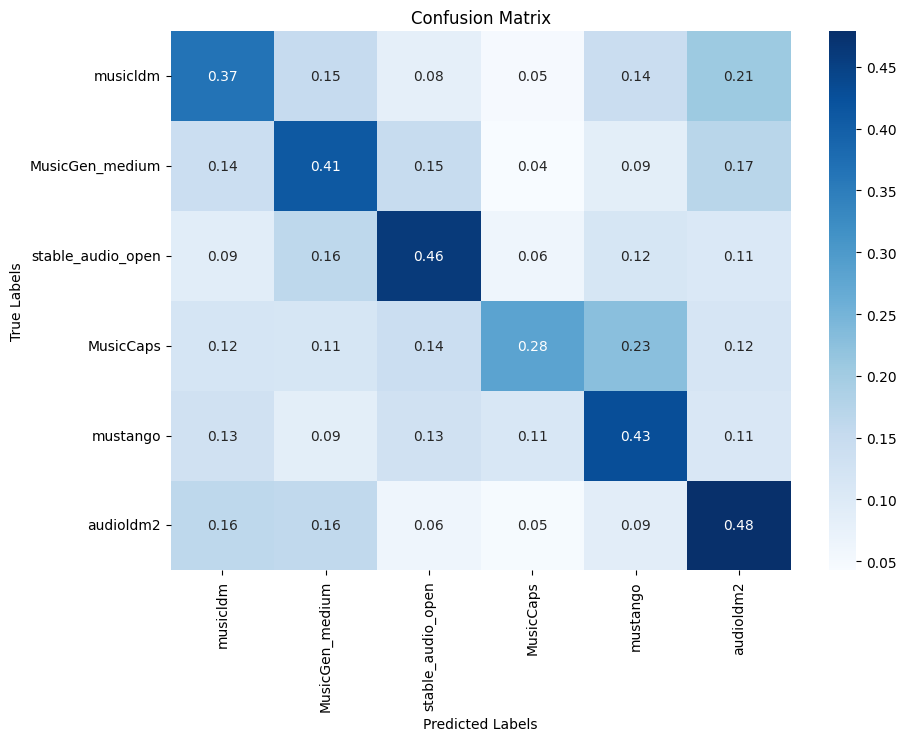
\includegraphics[width=1.11\linewidth]{Figures/ConfusionMatrixClosedSet.png}
        \caption{Confusion Matrix - Closed-Set}
        \label{fig: Closed-Set}
    \end{subfigure}%
    \hfill
    \begin{subfigure}[b]{0.32\textwidth}
        \centering
        % Questo era il tuo placeholder, ora usa l'immagine reale
        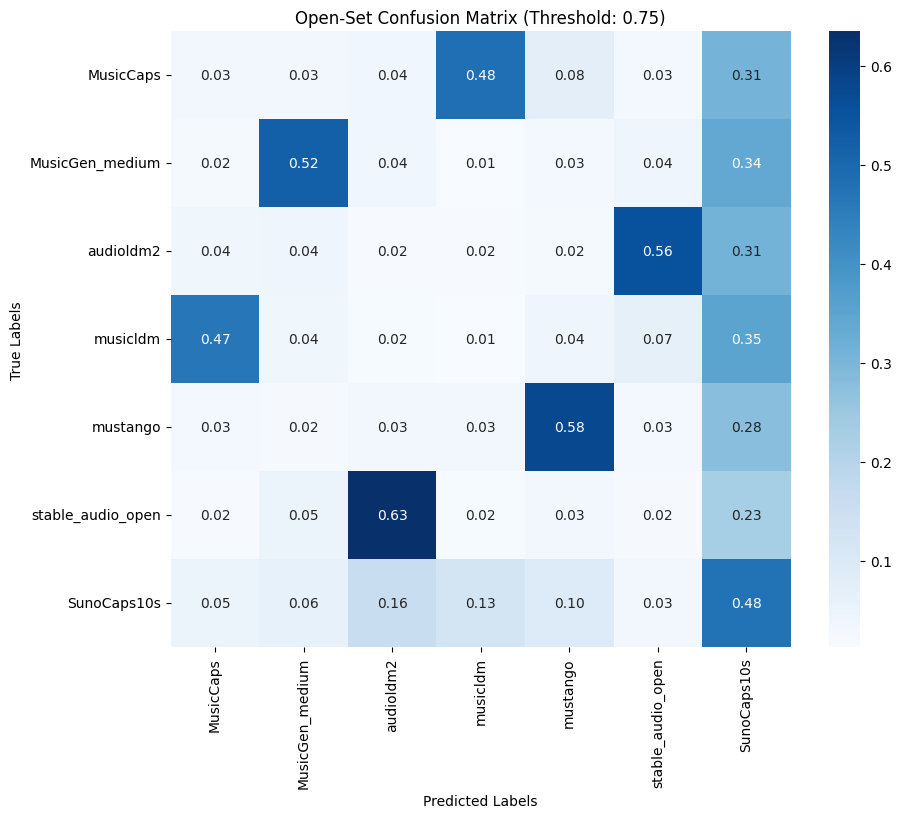
\includegraphics[width=\linewidth]{Figures/ConfusionMatrixOpenSetThreshold.PNG} % <--- Sostituisci con il nome reale della tua sesta figura
        \caption{Confusion Matrix - Open-Set Threshold}
        \label{fig: Open-Set Threshold}
    \end{subfigure}%
    \hfill
    \begin{subfigure}[b]{0.32\textwidth}
        \centering
        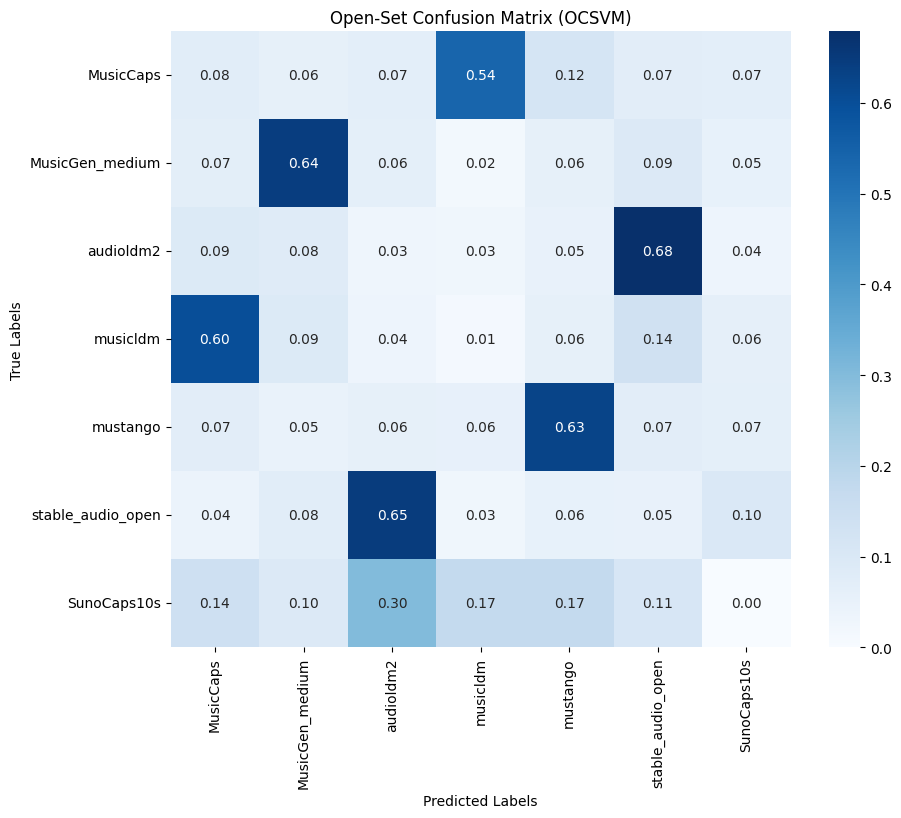
\includegraphics[width=\linewidth]{Figures/ConfusionMatrixOpenSetSVM.PNG}
        \caption{Confusion Matrix - Open-Set SVM}
        \label{fig: Open-Set SVM}
    \end{subfigure}

  
\label{fig:all_conf_matrices} % Didascalia generale per tutte le

\end{figure*}
    
\begin{figure*}
    \vspace{0.8em} % <--- Spazio verticale tra le due righe di figure

    % --- Seconda Riga: Tre Figure ---
    \begin{subfigure}[b]{0.32\textwidth}
        \centering
        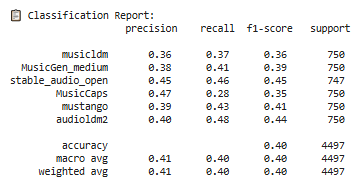
\includegraphics[width=\linewidth]{Figures/ReportClosedSet.PNG}
        \caption{Classification Report Closed-Set}
        \label{fig: Closed-Set Report}
    \end{subfigure}%
    \hfill
    \begin{subfigure}[b]{0.32\textwidth}
        \centering
        % Questo era il tuo placeholder, ora usa l'immagine reale
        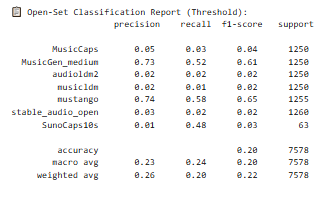
\includegraphics[width=\linewidth]{Figures/OpenSetThreshold.PNG} % <--- Sostituisci con il nome reale della tua sesta figura
        \caption{Classification Report Open-Set Threshold} % <--- Aggiorna la didascalia
        \label{fig: Open-Set Threshold Report}
    \end{subfigure}%
    \hfill
    \begin{subfigure}[b]{0.32\textwidth}
        \centering
        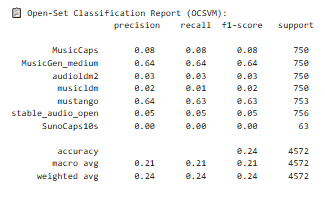
\includegraphics[width=\linewidth]{Figures/OpenSetSVM.PNG}
        \caption{Classification Report Open-Set SVM}
        \label{fig: Open-Set SVM Report}
    \end{subfigure}
\\
    \caption*{Figure: Confusion Matrices and Classification Reports for Different Models and Configurations} %
\label{fig:all_conf_matrices} % Didascalia generale per tutte le figure
\end{figure*}

Traditional text classification models operate under the closed-set assumption, where all classes present during testing were also observed during training. However, real-world scenarios are inherently open-set, meaning that the system could encounter data belonging to unseen or unknown classes; this translates to encountering captions from a generative model that was not part of the training dataset. 

The experimental evaluation of text classification across a dataset characterized by high semantic similarity between classes revealed distinct performance profiles for closed-set and open-set methodologies. In the initial closed-set scenario, a BERT-based classifier achieved moderate accuracy, with notable misclassifications between semantically proximate classes, such as MusicCaps frequently being mistaken for Mustango. This indicated the inherent challenge posed by the subtle distinctions within the caption data. Transitioning to open-set classification utilizing a softmax probability threshold (set at 0.75), the model demonstrated a partial capability to identify "unknown" samples (SunoCaps), achieving a recall of 0.48 for this novel class. However, this came at a significant cost: the recall for several known classes dramatically decreased (e.g., MusicCaps recall plummeted from 0.28 to 0.03), as a substantial portion of genuinely known instances were misclassified as "unknown" due to their maximum predicted probability falling below the defined threshold. This behavior is directly attributable to the high semantic overlap among known classes, leading to reduced model confidence in distinguishing them, and consequently, a tendency for uncertain predictions to be shunted to the "unknown" category. The One-Class SVM (OCSVM) approach, applied to BERT embeddings for open-set detection, exhibited a marked improvement in correctly classifying known instances, with significantly higher recall rates across some known classes (e.g., MusicGen\_medium to 0.64 from 0.52). The OCSVM proved highly effective at retaining known samples within their respective categories, suggesting that it learned a more robust boundary for the in-distribution data. However, this robustness came at the severe expense of novelty detection: the OCSVM virtually failed to identify any true "unknown" (SunoCaps) samples, yielding a 0.00 recall for this class. This outcome strongly implies that the BERT embeddings of the "unknown" SunoCaps captions lie within the semantic manifold learned by the OCSVM from the known data, rendering them indistinguishable as outliers. Collectively, these results underscore the formidable challenge of open-set text classification in datasets with high inter-class semantic similarity, highlighting a persistent trade-off between accurate known-class discrimination and robust unknown-class detection across different methodological paradigms.

We have several critical insights from these classification experiments:
\begin{itemize}
    \item Semantic similarity is a core challenge: the most significant learning is that the high semantic similarity among the captions within and across your known classes is the fundamental bottleneck. This inherent ambiguity makes it difficult for any model to achieve high confidence or clear separation, leading to misclassifications even in a closed-set scenario.

    \item Open-Set Classification involves inherent trade-offs: there's a clear tension between accurately classifying known instances and effectively detecting unknown ones.
    Threshold-based approach: prioritized detecting some unknown samples, but at the expense of misclassify many known samples as unknown (due to low confidence thresholds). 
    OCSVM approach: prioritized accurate classification of known samples, drastically reducing misclassifications of known as unknown. However, it failed almost entirely at identifying true unknown samples. It acted as a "more precise" known-class classifier but was "blind" to novelty that fell within the known data's semantic space.

    \item BERT embeddings offer rich semantic representations, but they're not a silver bullet for novelty detection. While they capture context well, they don’t explicitly encode how "known" or "unknown" a sample is, making it difficult for simple models like one-class SVMs to distinguish anomalies when semantic content is similar. This highlights the need for carefully selected and tuned downstream detection methods, especially in complex open-set scenarios.

    \item The "unknown" class is not truly out-of-distribution (semantically): The most crucial learning about SunoCaps "unknown" class is that, based on the OCSVM's performance, its captions are not sufficiently distinct (in the BERT embedding space) from known classes to be considered true semantic outliers. This implies that if you need to detect these specific "unknowns," you will likely require more sophisticated open-set detection algorithms or a different definition of "unknown" that captures features truly absent from your training data.
\end{itemize}

We learned that classifying these music captions, particularly in an open-set context, is hard, due to their semantic proximity. The choice of open-set method critically dictates the trade-off between identifying known classes accurately and recognizing genuinely novel content.


\section{Conclusion and Future Work}

Our results demonstrate the effectiveness of fine-tuned BERT in discriminating between known generative sources and highlight the capabilities and limitations of each open-set strategy in identifying novel, unseen sources. In essence, this project underscored the profound challenges of text classification in a domain characterized by high semantic similarity across classes, leading to the observed lower performance metrics. The closed-set evaluation, while showing moderate discriminative power, consistently revealed inherent ambiguities between known generative sources. Crucially, our exploration into open-set classification revealed a critical trade-off: the threshold-based approach offered a modest ability to identify 'unknown' samples but significantly hampered the accurate classification of known instances due to reduced model confidence. Conversely, the One-Class SVM (OCSVM) method drastically improved the precision of known-class identification, yet it proved largely ineffective at recognizing truly novel sources, as their BERT embeddings often fell within the learned manifold of known data. These implications collectively highlight the inherent difficulty in performing robust open-set classification when the 'unknown' distribution strongly overlaps with the 'known' in the feature space. 

Looking to the future, this project lays the groundwork for several critical avenues of research. Future work should involve leveraging the full dataset for training, implementing more sophisticated data pre-processing techniques to better normalize and semantically enrich captions, conducting deeper correlation analysis to quantitatively map semantic relationships between generative sources. 
Other options can lead to the need for open-set algorithms that go beyond simple feature extraction, focusing explicitly on modeling “frontiers” or identifying “novelty” \cite{hendrycks2018baselinedetectingmisclassifiedoutofdistribution}.

Furthermore, strategies like data augmentation \cite{article} for underrepresented 'unknown' classes or dynamic class weighting \cite{9324926} could mitigate label imbalance. Finally, exploring different state-of-the-art transformer models for text classification, including larger or specialized architectures, or even venturing into multimodal approaches that incorporate audio features, promises to unlock more robust detection of novel generative content. 

This is just the beginning of what the future state-of-the-art could and will do to optimize the detection and classification of generated musical content.

\nocite{*}
\bibliographystyle{plain}  % oppure ieee, alpha, apalike, ecc.
\bibliography{bibliography} % ref
\end{document}

